% Stage Report I (English). Build on LM2 (two passes), in docs/report/:
%   export PATH=/data6/jinxinhao/texlive/2026/bin/x86_64-linux:$PATH && pdflatex stage_report_1.tex
\documentclass[11pt]{article}
\usepackage[margin=1in]{geometry}
\usepackage{amsmath,amssymb}
\usepackage{booktabs}
\usepackage{graphicx}
\usepackage{xcolor}
\usepackage[hidelinks]{hyperref}
\emergencystretch=3em

\title{\bfseries Rare Nuclei on PanNuke Are a Detection Problem:\\
Diagnosis, Two Failed Data-Side Fixes, and a\\ Counterfactual Stress-Test Evaluation\\[6pt]
\large Stage Report I (Course Project bdd26)}
\author{}
\date{September 28, 2026}

\begin{document}
\maketitle

\begin{abstract}
On PanNuke, swapping backbones moves mean panoptic quality (mPQ) by only 1--2 points, while the
\emph{Dead} (apoptotic) class stagnates at PQ $\approx$ 0.13--0.18 for every published model. This
stage report asks why, and whether recent ``new paradigms'' (pathology vision--language models
and controllable generative models) can address either the rare-class deficit or robustness
evaluation. We first reproduce two baselines under the official 3-fold protocol (HoVer-Net
0.456 mPQ, CellViT-UNI 0.500) and add a third evaluator, HoVer-NeXt-T (0.458), after diagnosing
that our port's original 0.358 was a decoding artifact, not a model gap. Second, we show the Dead
deficit is concentrated in \emph{detection}, not classification: 38.5\% of Dead ground-truth
nuclei receive no overlapping prediction, and inside those missed nuclei the foreground head is
silent (mean nuclear-probability 0.16) while the type head assigns P(Dead)$\approx$0.26. Third,
under a pre-registered multi-seed protocol, four interventions are null or harmful: post-hoc
re-typing with a pathology VLM (CONCH), training-free missed-nucleus recovery, class-weighted and
size-weighted foreground losses, and, on the data side, failure-driven copy-paste (Dead PQ
$-0.031$) and in-context diffusion synthesis with self-consistent labels (mPQ unchanged).
Fourth, we build a three-architecture $\times$ three-dataset zero-shot cross-domain benchmark
(CoNIC, MoNuSAC, PUMA) and \emph{PanNuke-CF}, a counterfactual test set that re-renders fixed
PanNuke labels under interventions on tissue context and stain. Counterfactual stress
\emph{inverts} the real cross-domain ranking (Spearman $-0.89$ across 6 evaluator points;
$-1.00$ on architecture means): an axis decomposition shows real between-architecture transfer
differences live almost entirely on the detection axis, which label-fixed rendering cannot
stress by construction, while on the typing axis, which it does stress, counterfactual ranking
agrees with real transfer. We conclude counterfactual rendering is a valid \emph{typing} stress
test but not a transfer surrogate, and that the Dead detection deficit is architectural: it is
robust to every loss-level and data-level intervention we tested, and follows the models
out-of-domain (Dead PQ $\leq 0.006$ on PUMA for all three architectures).
\end{abstract}

\section{Introduction}
\label{sec:intro}

Nuclei instance segmentation and classification is a standard workload in computational
pathology, and PanNuke~\cite{gamper2019pannuke} its standard benchmark: 205,000 annotated nuclei
across 19 tissues, evaluated by tissue-averaged mean panoptic quality (mPQ). The published
leaderboard is lopsided: five years of architectural progress compress into
$\sim$1--2 mPQ points (HoVer-Net~\cite{graham2019hovernet} 0.463 $\rightarrow$
CellViT-SAM-H~\cite{horta2024cellvit} 0.498 $\rightarrow$ best current models
$\approx$0.51), while the \emph{Dead} (apoptotic bodies) class stays at PQ
0.13--0.18 and touching-nucleus merge/split errors persist. Two recent paradigm families
promise more than backbone engineering: pathology vision--language models
(VLMs)~\cite{lu2024conch} as priors for type classification, and controllable generative
models~\cite{le2025pixcell} as ``tissue simulators'' that can synthesise targeted training data
or re-render evaluation images under interventions.

This project was organised as three pre-registered pillars with explicit go/no-go rules, on the
logic that negative results are only useful if their acceptance criteria are fixed in advance:
\textbf{A}~--- language-anchored typing (attack rare-class \emph{classification} with the CONCH
text space); \textbf{B}~--- failure-driven synthesis (attack Dead/small-nucleus \emph{detection}
with generated data); \textbf{C}~--- evaluation (attack robustness measurement with real
cross-domain transfer plus a counterfactual test set). All three pillars have now closed; this
report documents what was found. Its contributions:

\begin{enumerate}
\item \textbf{Reproduction under a single strict protocol} (Sec.~\ref{sec:setup}): HoVer-Net,
CellViT-UNI, and HoVer-NeXt-T trained/evaluated identically on the official 3-fold split,
last-checkpoint, validation-tuned decodes only. Along the way we quantify how much a released
evaluation recipe (16 stochastic colour-TTA views + thresholds tuned on the \emph{test} fold)
inflates reported numbers (Sec.~\ref{sec:baselines}).
\item \textbf{A decomposition of the Dead deficit} (Sec.~\ref{sec:diagnosis}): it is a
\emph{detection} failure concentrated in small and isolated nuclei, invisible to the foreground
head but partially ``seen'' by the type head---which is exactly why every typing-side
intervention fails.
\item \textbf{Pre-registered negative results} (Secs.~\ref{sec:pillarA}, \ref{sec:pillarB}):
CONCH re-typing, training-free recovery, loss re-weighting (3 seeds), failure-driven
copy-paste, and in-context diffusion synthesis are all null or harmful, with seed-noise
calibration that says which effect sizes would have been believable.
\item \textbf{A $3{\times}3$ architecture $\times$ dataset zero-shot cross-domain benchmark}
(Sec.~\ref{sec:external}), including PUMA as the only sizable external source of apoptotic-body
Dead labels we could find, and a conversion/verification pipeline for CoNIC and MoNuSAC.
\item \textbf{PanNuke-CF}, a label-fixed counterfactual rendering benchmark
(Sec.~\ref{sec:cf}), with a validity analysis that reaches a mechanistic verdict: counterfactual
appearance stress cannot probe detection (by construction) and therefore \emph{inverts} the
real transfer ranking at the mPQ level, while remaining valid as a typing stress test.
\end{enumerate}

Everything is one codebase; every number below comes from the same evaluator, which was checked
bit-exact against the official PanNuke-metrics implementation (whose published
\texttt{class\_stats.csv} has a column-swap bug we document in the repository).

\section{Related Work}
\label{sec:related}

\paragraph{PanNuke models.} HoVer-Net~\cite{graham2019hovernet} introduced the
horizontal--vertical watershed decode still used (in variants) by most successors.
CPP-Net~\cite{cppnet}, HoVer-NeXt~\cite{hovenext}, CellViT~\cite{horta2024cellvit} and its
successors (LKCell, CellVTA, CellViT++~\cite{horta2025cellvitpp}), and
PromptNucSeg~\cite{promptnucseg} populate the 0.46--0.51 mPQ band. Publicly released per-fold
weights exist for only some of these; several official checkpoints (e.g.\ HoVer-Net's) were
trained on all folds and can only serve as pipeline sanity checks, never as test
results---we enforce this distinction throughout.

\paragraph{Pathology foundation models and VLMs.} Frozen pathology foundation models do not
automatically beat ImageNet CNNs on dense tasks~\cite{mindthegap}, and the pathology VLM
CONCH~\cite{lu2024conch} is on par with pure-visual models for dense prediction while providing
an aligned text space. Pure prompt-based interfaces fail badly on nuclei (SAM3-style prompting
achieves $<10\%$ mIoU on PanNuke-type tasks), and the closest prior work (PromptNu, MONCH)
either lacks an official PanNuke configuration or reports only semantic segmentation. We found
no prior work combining a pathology VLM text space with instance segmentation under the official
PanNuke protocol.

\paragraph{Generative augmentation and stress tests.} Synthesis for nuclei segmentation has
been reported to help \emph{rare classes} (DiffMix, HistoSmith, NucleiMix~\cite{nucleimix})
but never, to our knowledge, under the official 3-fold PanNuke protocol with mPQ; existing
studies use non-standard splits and Dice/AJI/F1. Counterfactual stress testing of imaging
models has been demonstrated in radiology~\cite{cfstress}; we are not aware of an instance
segmentation analogue. PixCell~\cite{le2025pixcell} (with its Cell-ControlNet) is the
strongest openly available controllable nuclei generator, and is the base of both our synthesis
experiments and our counterfactual renderer.

\section{Experimental Setup}
\label{sec:setup}

\paragraph{Data and protocol.} PanNuke folds 1--3 with the official assignment (train/val/test
$=1/2/3$, $2/1/3$, $3/2/1$); all numbers are 3-split means of \emph{last-checkpoint} models with
no test-based early stopping. External datasets (Sec.~\ref{sec:external}) are zero-shot: class
mappings to the 5 PanNuke classes are fixed per dataset, absent classes are excluded from mPQ
per the official protocol.

\paragraph{Metrics.} Official tissue-averaged mPQ/bPQ (bit-exact reimplementation of
PanNuke-metrics), strict mPQ (FPs on classes absent from an image are penalised rather than
ignored), AJI/AJI$^+$, detection $F_d$ and classification $F_c$ (12\,px centroid matching), and
an IoU-0.5 error decomposition (matched / merged / missed-no-overlap / missed-poor-shape /
split, per class). TTA (8 dihedral views with HV-channel remapping) is reported separately.

\paragraph{Noise calibration (used for every verdict).} Across 3 seeds of the identical
CellViT-UNI recipe: seed std is 0.0021 mPQ but \textbf{0.0074 Dead PQ}, and the image-bootstrap
CI half-width on Dead is 0.02--0.03. Rules we enforce: single-seed Dead changes below
$\sim$0.01--0.015 are noise; every intervention verdict is a 3-seed (or multi-fold) statement
with paired, tissue-stratified image-bootstrap 95\% CIs; validation-fold decisions only.

\subsection{Baselines}
\label{sec:baselines}

\begin{table}[t]
\centering\small
\caption{Baselines under the official 3-fold protocol (3-split mean; last checkpoint; no TTA,
TTA in brackets). ``Published'' = paper-reported numbers under their own recipes.}
\label{tab:baselines}
\begin{tabular}{lccc}
\toprule
Model & mPQ & bPQ & Dead PQ \\
\midrule
HoVer-Net (ours)            & .4564 [.4666] & .6613 [.6714] & .127 [.128] \\
\quad published             & .463 & .660 & .139 \\
CellViT-UNI (ours)          & .4995 [.5047] & .6654 [.6706] & .176 [.177] \\
\quad published (CellViT++) & .492 & .664 & .154 \\
HoVer-NeXt-T (ours)         & .4579 & .6367 & .136 \\
\quad published             & .477 & .656 & .154 \\
\bottomrule
\end{tabular}
\end{table}

Table~\ref{tab:baselines}: both classic baselines reproduce (HoVer-Net slightly below paper,
consistent with common reproductions; CellViT-UNI slightly above). HoVer-NeXt-T required
porting and initially scored 0.358 mPQ; ablations showed the \emph{predicted maps were fine}
and the loss was entirely in the decode. Its released 0.477 recipe averages 16 stochastic
spatial+\emph{colour} TTA views and tunes per-class thresholds \emph{on the test fold}. We
instead use its own validation decode (flat fg/seed thresholds) tuned on each split's
\emph{validation} fold---the same protocol as our other baselines---yielding 0.4579. The gap
(0.458 vs 0.477) is a measure of what test-side tuning + stochastic colour TTA buy, and we flag
that recipe differences of this size (0.02 mPQ) are larger than most leaderboard gaps.
HoVer-NeXt-T earns its place as our third evaluator through a \emph{different error profile}:
lowest merge rate of the three (0.096--0.101 vs $\approx$0.14 for HoVer-Net), higher
missed-background.

\section{Pillar A: The Dead Deficit Is a Detection Deficit}
\label{sec:pillarA}

\subsection{CONCH semantics live at the context scale (feasibility)}
Zero-shot CONCH classification of ground-truth nuclei: tight crops are near chance (32\,px:
0.27), full-context patches with radius-restricted attentional pooling reach balanced accuracy
0.695 (R\,=\,32\,px, one forward pass per patch), with LLM morphology descriptions beating bare
class names by 8--11 points. Dead is the \emph{most} text-recognisable class (recall 0.88) yet
the worst class for segmentation models---but at natural prevalence its zero-shot precision is
$\approx$0.10, so it can only be a complementary signal. Text-anchored initialisation of a
linear head helps only in the few-shot regime ($\le$25 nuclei/class); with full PanNuke labels
it is irrelevant. This redirected pillar A from classification to detection.

\subsection{In-pipeline re-typing: null}
Fusing CONCH (zero-shot or linear-probe) into the type decision of CellViT-UNI, with all knobs
tuned on the validation fold (Table~\ref{tab:retype}): no configuration beats the pipeline's own
seg-vote typing, and the recalibration control matches the best fusion. With TTA, validation
tuning picks $\alpha=0$ for both fusions.

\begin{table}[t]
\centering\small
\caption{Post-hoc re-typing on CellViT-UNI, split 1 (test fold 3).}
\label{tab:retype}
\begin{tabular}{lccc}
\toprule
Method & val mPQ & test mPQ & test Dead PQ \\
\midrule
seg vote (pipeline)              & .4835 & .4951 & .142 \\
+ class-bias recalibration       & .4873 & .4953 & .135 \\
$\times$ CONCH zero-shot ($\alpha{=}.1$) & .4835 & .4938 & .141 \\
$\times$ CONCH linear ($\alpha{=}.3$)    & .4836 & .4920 & .141 \\
CONCH linear alone               & .3645 & .3821 & .145 \\
\bottomrule
\end{tabular}
\end{table}

\subsection{Training-free recovery: null}
A 96-configuration sweep over foreground mixing, dead-prior boosting, blob thresholds and
orphan recovery on the raw NP/HV/TP maps (3 splits; selection on validation): every family lands
within $\pm0.0004$ test mPQ of the threshold-only control. The missed Dead nuclei are not
recoverable from this model's outputs.

\subsection{Loss-side ablations: null or a trade}
Pixel-weighted foreground CE on split 1 with 3-seed baselines: Dead-pixel weight $\times$11 (M1)
null; fully balanced sampler (C1) null; small-nucleus weight $\times$6 (M2) looked promising in
one seed ($+0.0042$ test mPQ, CI excluding 0) but across 3 seeds is mPQ $-0.0010$
$[-0.0043,+0.0022]$ with a \emph{significant} bPQ loss $-0.0024$ $[-0.0048,-0.0002]$ and a
non-significant Dead gain $+0.0108$ $[-0.0021,+0.0238]$---a trade, not a contribution, and a
clean demonstration that single-seed mPQ effects below $\sim$0.004 on this benchmark are seed
luck.

\subsection{Diagnosis: where Dead performance is lost}
\label{sec:diagnosis}

\begin{table}[t]
\centering\small
\caption{Error decomposition of CellViT-UNI on fold 3 (IoU 0.5; fraction of GT nuclei).}
\label{tab:decomp}
\begin{tabular}{lcccccc}
\toprule
GT class & matched & merged & missed & miss (shape) & split & type$\mid$matched \\
\midrule
Neoplastic   & .811 & .048 & .092 & .040 & .009 & .905 \\
Inflammatory & .849 & .046 & .079 & .023 & .004 & .817 \\
Connective   & .752 & .038 & .153 & .044 & .013 & .794 \\
Dead         & \textbf{.470} & .089 & \textbf{.385} & .048 & .008 & .690 \\
Epithelial   & .837 & .042 & .075 & .036 & .011 & .930 \\
\bottomrule
\end{tabular}
\end{table}

Table~\ref{tab:decomp}: 38.5\% of Dead nuclei have \emph{no overlapping prediction at all}
(other classes 8--15\%), while Dead type-when-matched is 0.69---the loss is detection-first.
Inside the missed Dead nuclei the foreground head is silent (mean NP probability 0.164; fires in
17\% of them) yet the type branch assigns P(Dead)\,$\approx$\,0.26 (vs $\approx$0.01 for missed
nuclei of other classes): the network ``sees'' dead material that the foreground head drops.
Size drives much of it (Dead median area 107\,px vs 368 for other classes; 24\% of Dead are
$<$60\,px vs 6\%), but an appearance effect survives size stratification: large Dead
($>$200\,px) are missed 6$\times$ more often than large nuclei of other classes (0.214 vs
0.035). Qualitatively (Fig.~\ref{fig:dead}), missed Dead are karyorrhectic fragments,
chromatin-poor eosinophilic bodies, and ambiguous annotations. Conclusion: fix detection or the
data---which defines pillar B.

\begin{figure}[t]
\centering
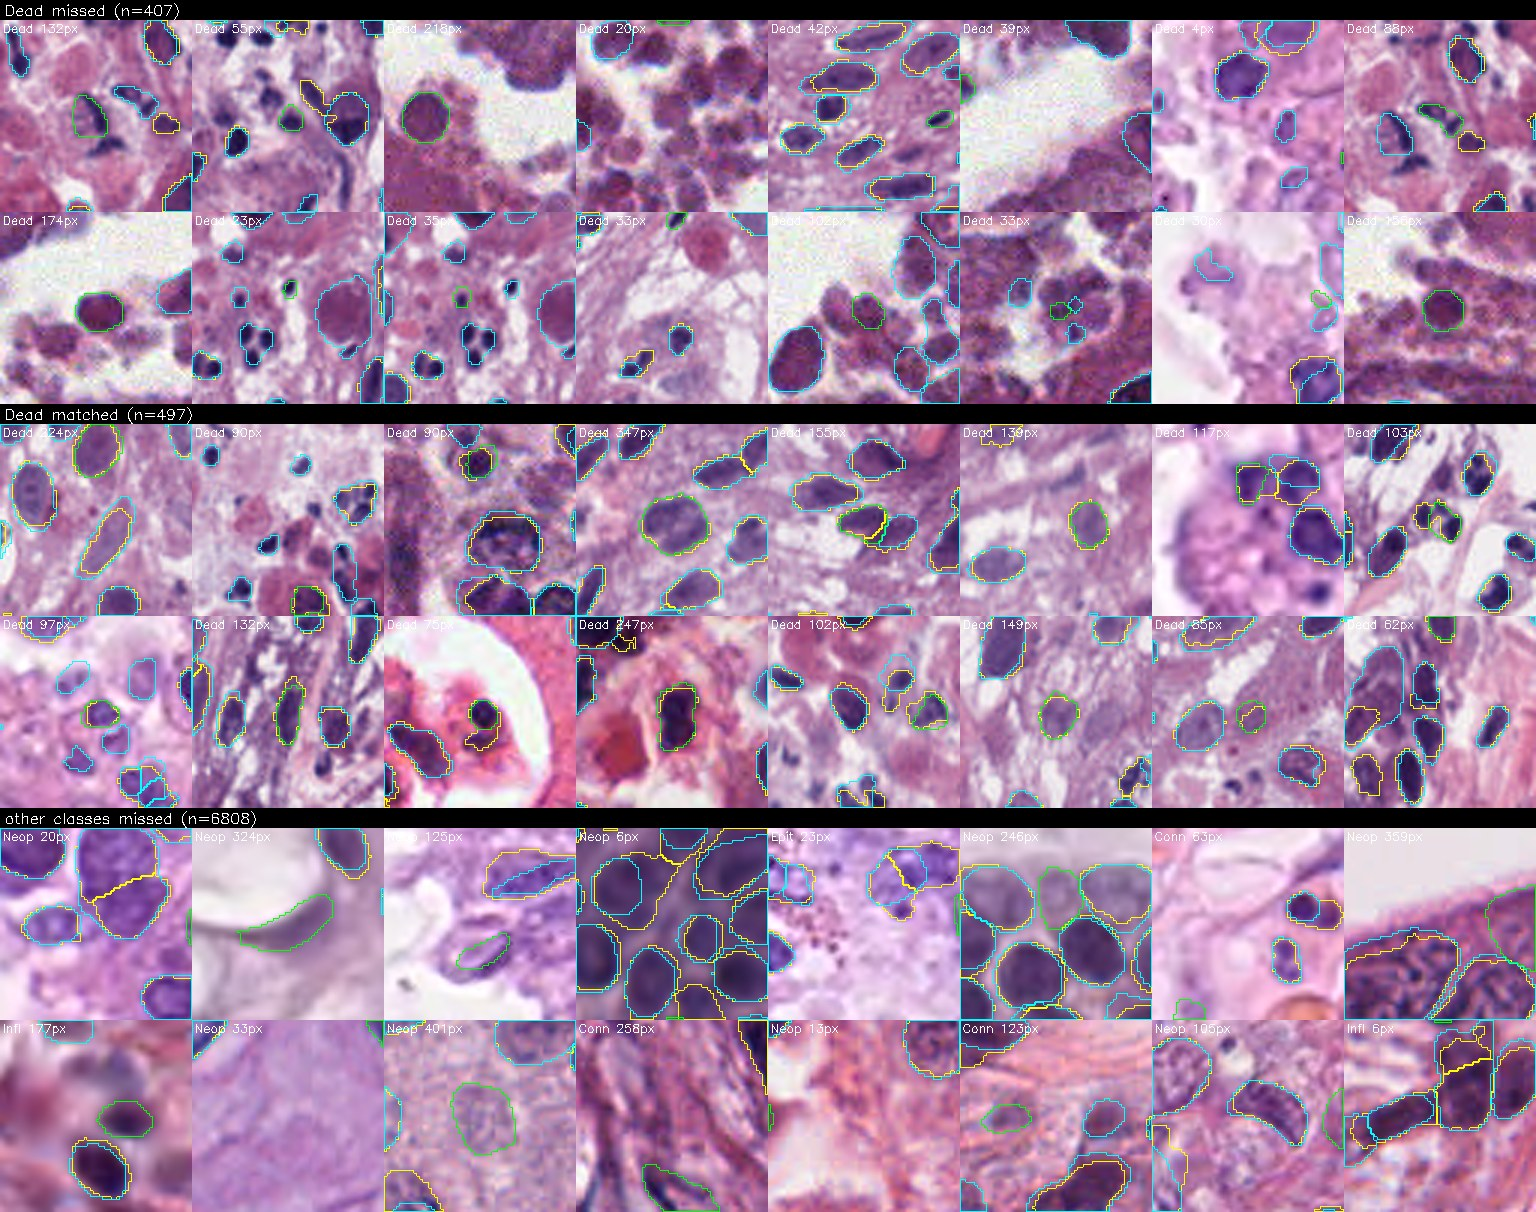
\includegraphics[width=0.86\linewidth]{figs/dead_missed.jpg}
\caption{Dead ground-truth nuclei (green) vs.\ predictions (yellow), CellViT-UNI on fold 3:
missed Dead are tiny dark fragments and chromatin-poor apoptotic bodies that carry no foreground
response.}
\label{fig:dead}
\end{figure}

\section{Pillar B: Failure-Driven Synthesis Does Not Fix Detection Either}
\label{sec:pillarB}

\subsection{What failure layouts look like}
Out-of-fold failure mining (split-2 model on fold 1; identical patterns on fold 3 test):
missed Dead are \emph{isolated}---Dead with zero touching neighbours have miss rate 0.39--0.42
($\sim$90\% of all Dead), and missed Dead touch another nucleus in $<$5\% of cases. Merges are
an intra-class cluster phenomenon (73--82\% of merged Dead touch another Dead: karyorrhexis
fragments). Cross-class touching, the intuitive hypothesis, is rare and not the failure mode.
The originally planned ``Dead glued to Neoplastic'' intervention was therefore replaced by
(1) isolated small-nucleus insertion into empty stroma and (2) dense same-class clusters.

\subsection{CP1: failure-driven copy-paste is harmful}
Donor nuclei (50--400\,px, Dead-weighted 0.4) pasted into nucleus-free stroma with 8\,px
clearance \emph{before} geometric/photometric augmentation (so pasted nuclei are augmented
identically; a v1 shortcut caught by visual review and fixed, alongside border-fragment and
unannotated-nucleus collisions). Result vs 3-seed baseline (split 1; test fold 3):
$\Delta$mPQ $+0.0009$ $[-0.0024,+0.0043]$ but $\Delta$Dead \textbf{$-0.0310$}
$[-0.0576,-0.0100]$ (TTA-consistent). The damage is in \emph{typing}, not detection: matched-Dead
type accuracy .690$\rightarrow$.609, confusion increases in both directions. The
validation fold, however, pointed the \emph{opposite} way on Dead ($+0.0235$): Dead PQ swings $\sim$0.05
between folds, the third independent confirmation of the noise rules. Interpretation:
transplanting real appearances into new contexts teaches ``small isolated nucleus in clean
stroma'' as a Dead-ish cue and blurs the type boundary.

\subsection{In-context synthesis (PixCell): from an appearance gap to a structural blocker}
PixCell-256 + Cell-ControlNet with real fold-1 masks as condition: placement is faithful
($\sim$95\% of mask objects rendered at the right place/size, median IoU 0.68) but the 20$\times$
generator has a structural appearance gap on 40$\times$ PanNuke (flat chromatin, $-24\%$
high-frequency content, size-biased under-rendering of large masks). LoRA adaptation (two
rounds, r16 and r8 with snapshot selection) made every image-space metric \emph{worse} and was
abandoned; a Reinhard LAB transfer to the paired real patch closes the colour gap
(OD-L1 0.072$\rightarrow$0.009). With the locked recipe (base model + paired context +
Reinhard), visual review of 32-image smokes passes (colour within $\sim$3/255 of paired real),
but review exposed a structural blocker: the ControlNet condition is a \emph{binary} mask and
the context embedding carries no class information, so the generator cannot render
class-targeted appearance---0 of 729 kept objects were teacher-typed Dead (P(Dead)
$\le 0.005$). Forcing donor-class labels would recreate exactly the CP1 failure (labels that
contradict appearance). SYN1 therefore used \emph{class-agnostic, teacher-self-consistent}
labels, which can only help through detection: 1146 synthetic images at 50\% mixing, exact
base recipe otherwise. Result (test fold 3): mPQ 0.4900 vs base 0.4951 (bottom of the 3-seed
range 0.4910--0.4951), Dead 0.1521 vs 0.1424 ($\approx$$+1$pt, at the edge of seed noise, with
PQ$^+$/DQ$^+$/SQ$^+$ all flat: the sliver of Dead gain is better type pairing, not better
segmentation) and Inflammatory $-1.0$--$1.6$pts. Per the pre-registered rule: null.

\begin{figure}[t]
\centering
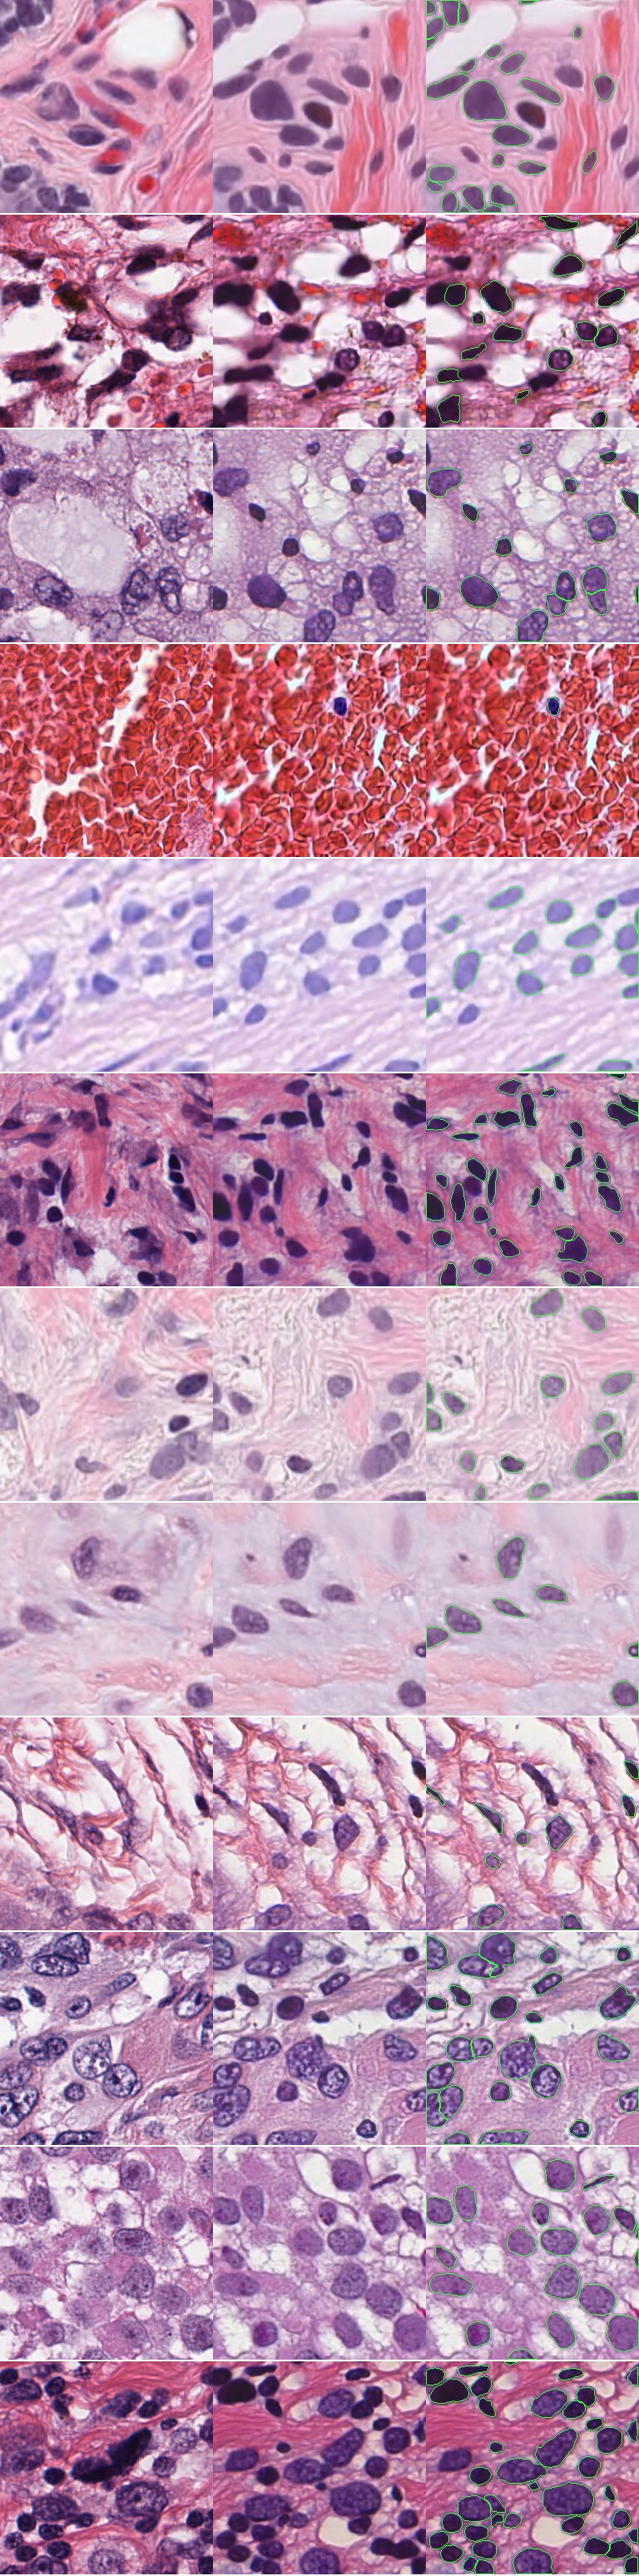
\includegraphics[width=0.30\linewidth]{figs/synth_v2.jpg}
\caption{SYN-v2 synthesis examples (real $|$ generated $|$ labels): with paired context +
Reinhard the appearance passes review, but the generator's binary-mask conditioning cannot
express class-targeted appearance (no generated object is readable as Dead).}
\label{fig:synth}
\end{figure}

\subsection{Pillar B verdict}
The Dead/small-nucleus detection deficit is not fixable by the data-side levers available
without retraining the generator's conditioning: real-appearance transplant (CP1) actively harms
Dead typing, and in-context synthesis with self-consistent labels (SYN1) is null. Together with
pillar A's nulls (re-typing, recovery, loss re-weighting), the deficit looks architectural.

\section{Pillar C: Cross-Domain and Counterfactual Evaluation}
\label{sec:pillarC}

\subsection{Real cross-domain zero-shot: $3{\times}3$}
\label{sec:external}

External sets, converted and montage-review-verified: \textbf{CoNIC} (19,476 tiles; the 112
patches sourced from PanNuke excluded; 20$\times\rightarrow$2$\times$ upsampled; classes
Inflam/Epith/Conn), \textbf{MoNuSAC} test (443 tiles; Inflam/Epith), \textbf{PUMA} melanoma
(3,278 tiles; all five PanNuke classes present, including 1,991 apoptotic$\rightarrow$Dead
nuclei---the only sizable external Dead supply we found; GT is HoVer-Net-initialised and
pathologist-corrected, so absolute recall has a ceiling that applies equally to all models).

\begin{table}[t]
\centering\small
\caption{Zero-shot cross-domain (3-split mean, no TTA). In-domain mPQ: CellViT 0.4995,
HoVer-Net 0.4564, HoVer-NeXt-T 0.4579.}
\label{tab:external}
\begin{tabular}{llccc}
\toprule
Model & Dataset & mPQ & bPQ & $F_d$ \\
\midrule
CellViT-UNI  & CoNIC   & .3351\,$\pm$.0037 & .5314 & .7816 \\
             & MoNuSAC & .2495\,$\pm$.0218 & .5616 & .7652 \\
             & PUMA    & .4518\,$\pm$.0031 & .7177 & .8831 \\
\midrule
HoVer-Net    & CoNIC   & .2610\,$\pm$.0061 & .5136 & .7669 \\
             & MoNuSAC & .0370\,$\pm$.0003 & .2756 & .3658 \\
             & PUMA    & .3203\,$\pm$.0139 & .7136 & .8714 \\
\midrule
HoVer-NeXt-T & CoNIC   & .2786 & .4811 & .725 \\
             & MoNuSAC & .1123 & .4025 & .628 \\
             & PUMA    & .3813 & .6888 & .848 \\
\bottomrule
\end{tabular}
\end{table}

Table~\ref{tab:external}: all models degrade, but differently. HoVer-Net nearly
\emph{collapses} on MoNuSAC ($F_d$ 0.37; per-split 0.26--0.78): a detection failure.
On PUMA no model collapses in detection ($F_d$ 0.85--0.88)---the loss there is \emph{typing}
(strict mPQ 0.31 vs mPQ 0.38 for HoVer-NeXt-T), and \textbf{Dead PQ is $\le$0.006 for all three
architectures} despite 1,991 apoptotic GT nuclei: the Dead failure mode follows the models
out-of-domain. TTA does not rescue transfer ($+0.005$ CoNIC, $-0.001$ MoNuSAC). Real domain
drop (in-domain minus mean external mPQ) ranks architectures CellViT 0.152 $<$ HoVer-NeXt-T
0.199 $<$ HoVer-Net 0.246, consistently on every dataset.

\subsection{PanNuke-CF: label-fixed counterfactual rendering}
\label{sec:cf}

\begin{figure}[t]
\centering
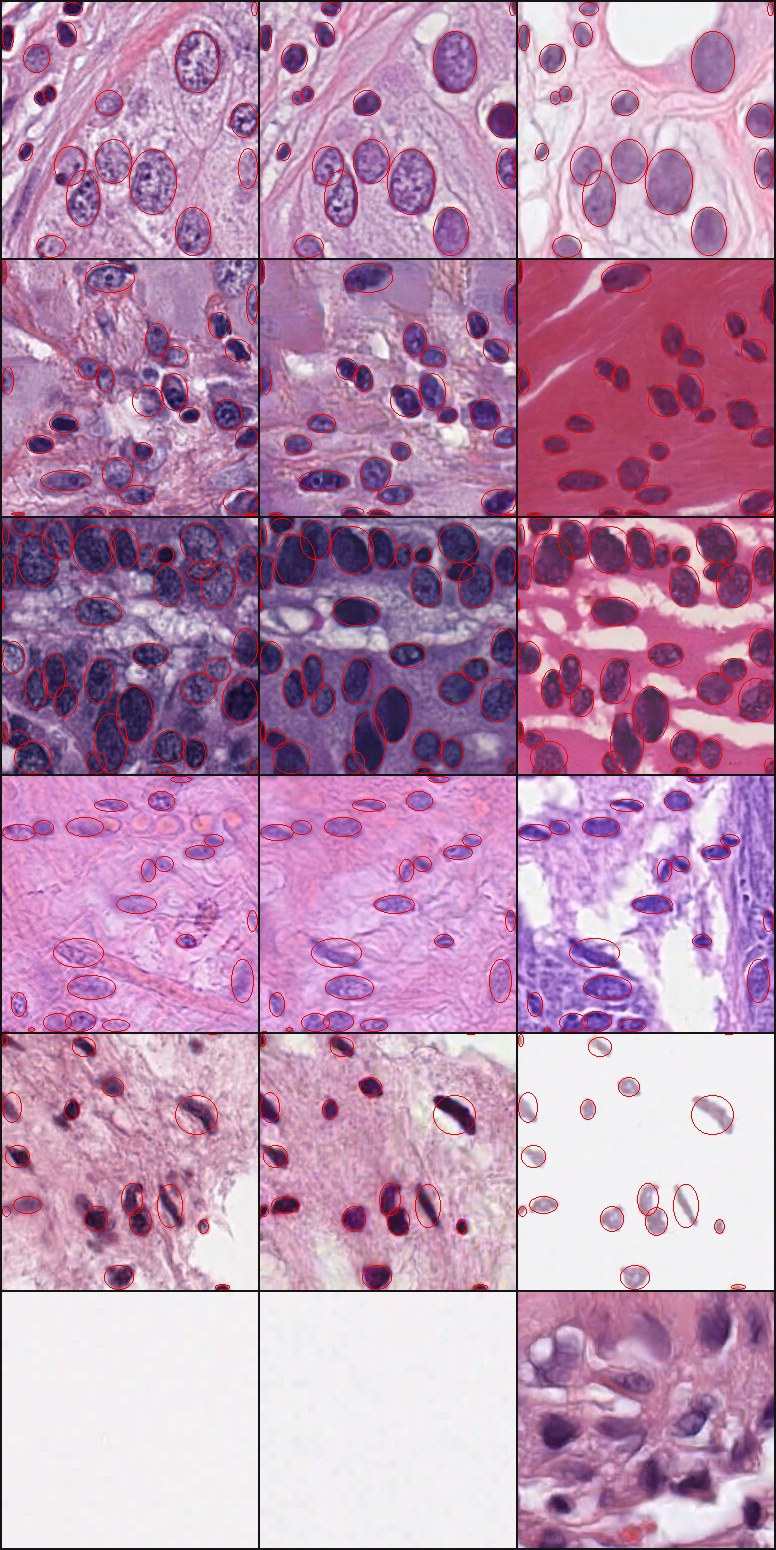
\includegraphics[width=0.42\linewidth]{figs/cf_arms.jpg}
\hfill
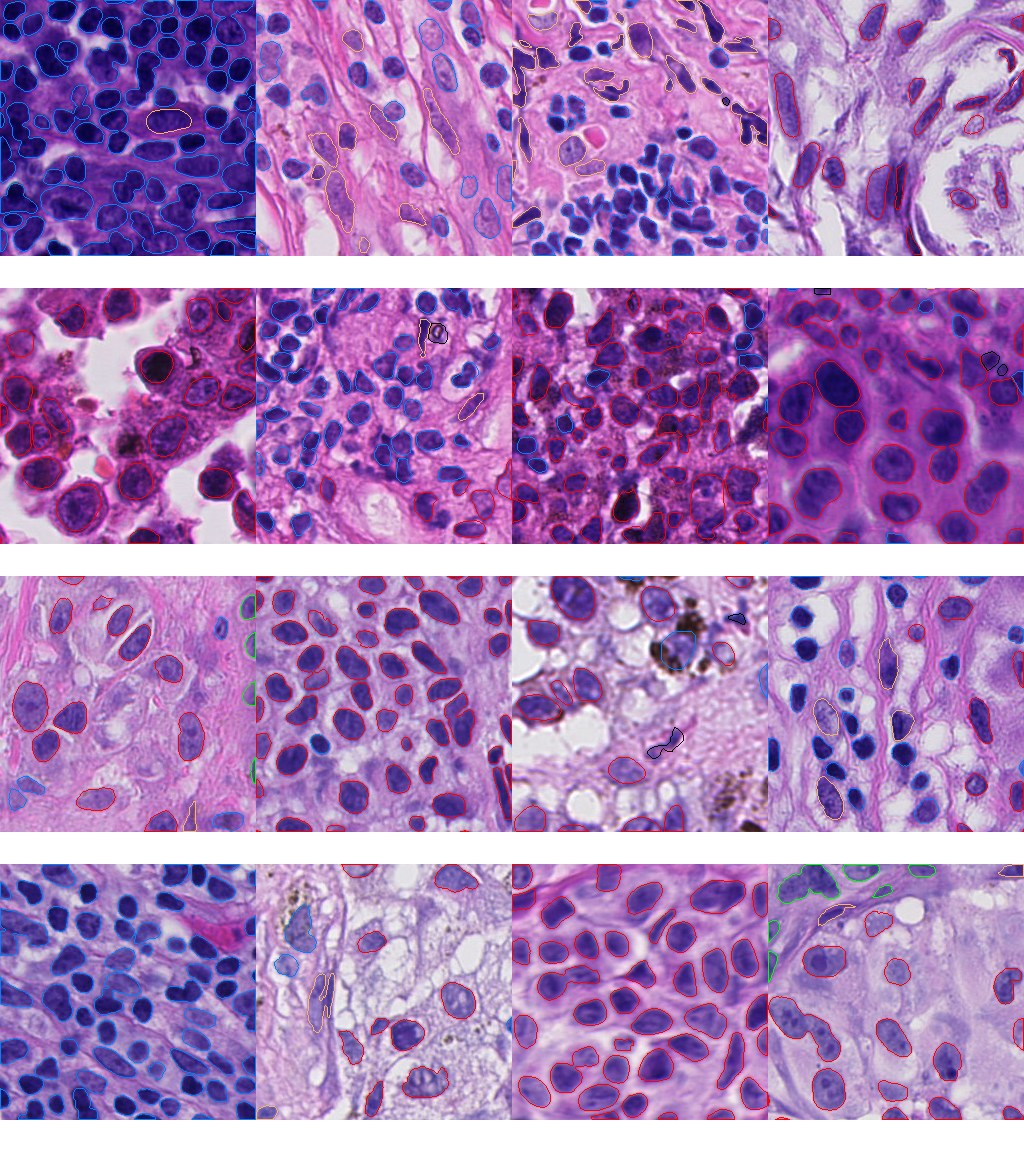
\includegraphics[width=0.42\linewidth]{figs/puma_gt.jpg}
\caption{Left: PanNuke-CF arms (same fold-3 GT labels re-rendered under context/stain
interventions). Right: PUMA ground truth (colour-coded classes; black outlines = apoptotic
Dead), the external set that supplies cross-domain Dead labels.}
\label{fig:cf}
\end{figure}

500 fold-3 patches with \emph{fixed GT labels} are re-rendered by the (frozen) generator under a
factorial appearance intervention---context \{paired, swapped-tissue\} $\times$ Reinhard target
\{self, donor\}---giving arms \texttt{control}/\texttt{stain}/\texttt{ctx}/\texttt{tissue},
plus the untouched \texttt{real} images and 3 generator-seed replicates of control for a noise
floor. Generator noise sits an order of magnitude below the intervention effects
(control-replicate mPQ std 0.002--0.006). Two calibration facts: generated \texttt{control} images are \emph{easier to
segment} than real (bPQ 0.78 vs 0.67) but carry \emph{type-inconsistent} appearance (strict mPQ
0.36 vs 0.45)---so CF comparisons are always arm-vs-control, never arm-vs-real; and blank
patches must be excluded (the context embedding is a content channel).

\begin{table}[t]
\centering\small
\caption{PanNuke-CF, architecture means over 2 splits (mPQ; paired $\Delta$ vs control mean in
brackets, image-bootstrap 95\% CI all exclude 0 except HoVer-NeXt-T stain).}
\label{tab:cf}
\begin{tabular}{lccccc}
\toprule
Architecture & real & control & stain & ctx & tissue \\
\midrule
CellViT-UNI  & .495 & .449 & .426 [$-$.023] & .259 [$-$.190] & .258 [$-$.191] \\
HoVer-Net    & .449 & .439 & .373 [$-$.066] & .300 [$-$.140] & .293 [$-$.146] \\
HoVer-NeXt-T & .456 & .425 & .417 [$-$.008] & .262 [$-$.163] & .261 [$-$.164] \\
\bottomrule
\end{tabular}
\end{table}

Context swap is a strong stressor (Epithelial PQ collapses by 0.24--0.43 while $F_d$ drops only
0.08--0.10: it destroys \emph{type} information), stain a mild one. The validation question is
whether these counterfactual drops predict \emph{real} cross-domain drops across evaluators.

\subsection{Validity: counterfactual stress inverts the real ranking}
\label{sec:validity}

Across 6 evaluator points (3 architectures $\times$ 2 splits), CF drop vs.\ real domain drop:
Spearman $\rho=-0.89$ for \texttt{ctx} (exact permutation $p=0.033$), $-0.89$ for
\texttt{tissue}, $+0.43$ n.s.\ for \texttt{stain}. On architecture means (the honest test; the
two splits of one architecture are near-duplicates) both ctx and tissue give $\rho=-1.00$: a
perfect inversion---the model most damaged by context swap in-domain (CellViT) is the most
robust real-domain transferrer, and vice versa.

\begin{table}[t]
\centering\small
\caption{Axis decomposition (architecture means): each drop split into detection ($F_d$) and
typing (bPQ$-$mPQ gap increase). Real between-architecture differences live on the detection
axis, where CF stress is architecturally homogeneous.}
\label{tab:axes}
\begin{tabular}{lcc|cc|cc}
\toprule
& \multicolumn{3}{c|}{Real (in-domain $-$ ext)} & \multicolumn{3}{c}{CF ctx (control $-$ ctx)} \\
Architecture & mPQ & $F_d$ & typing & mPQ & $F_d$ & typing \\
\midrule
CellViT-UNI  & .154 & \textbf{.007} & +.088 & .190 & .102 & +.082 \\
HoVer-Net    & .246 & \textbf{.163} & +.069 & .140 & .084 & +.034 \\
HoVer-NeXt-T & .199 & \textbf{.045} & +.085 & .163 & .090 & +.064 \\
\midrule
\multicolumn{7}{l}{\footnotesize Axis-matched rank agreement (all 6 points / architecture means):}\\
\multicolumn{7}{l}{\footnotesize\quad mPQ: $-0.89$ ($p{=}.033)$ / $-1.00$;\quad
detection $F_d$: $-0.83$ ($p{=}.058$) / $-1.00$;\quad typing: $+0.71$ / $\mathbf{+1.00}$.}\\
\bottomrule
\end{tabular}
\end{table}

Table~\ref{tab:axes} gives the mechanism. Real transfer differences between architectures
concentrate on the \emph{detection} axis (CellViT loses 0.007 $F_d$; HoVer-Net loses 0.163---its
MoNuSAC collapse), while typing-gap increase is similar for all (0.07--0.09). But label-fixed
rendering \emph{cannot} stress detection: the generator re-renders well-formed nuclei at fixed
positions, and indeed CF $F_d$ drops are homogeneous (0.08--0.10) across architectures with no
ordering information. Where CF \emph{can} apply stress---typing under context/stain
mismatch---its ranking agrees with real typing transfer ($\rho=+1.00$ on architecture means;
$+0.71$/$+0.83$ over all 6 points). Caveats: $n=3$ architectures (an arch-mean
$|\rho|=1$ has exact $p=1/3$; the defensible evidence is the perfect sign inversion across
3 architectures $\times$ 2 splits plus the axis mechanism), and real typing differences between
architectures are small (range 0.069--0.088) compared with detection differences (0.007--0.163).

\paragraph{Verdict.} PanNuke-CF is a valid \emph{typing stress test}---it ranks architectures'
typing robustness consistently with real transfer---but it is \emph{not} a transfer surrogate:
used as one, it inverts the ranking, because its blind spot (detection) is exactly where real
transfer differences live. Appearance-only counterfactuals inherit this limitation by
construction; probing detection robustness requires interventions on \emph{layout} (density,
clutter, artefact), not appearance.

\section{Discussion}
\label{sec:discussion}

\paragraph{Why all three pillars went negative, together.} The pillars shared one implicit
hypothesis---that Dead performance is limited by information (language priors) or data
(synthetic examples) rather than by the detection architecture. The diagnosis says otherwise:
missed Dead nuclei produce no foreground response at 83\% pixel level, the type branch
already ``sees'' them, and neither language-side fusion, post-hoc recovery, loss re-weighting
(3 seeds), real-appearance transplant, nor in-context synthesis with self-consistent labels
moved detection. The deficit is consistent with the resolution/architecture of the NP head at
40$\times$, a hypothesis we have not yet tested architecturally (e.g.\ higher-resolution
foreground supervision) and which is the main open direction.

\paragraph{Evaluation methodology.} Three lessons, each with evidence: (1) seed noise on PanNuke is
class-dependent (mPQ 0.002 vs Dead 0.007) and validation-fold Dead signals can point opposite
to test (CP1: $+0.024$ vs $-0.031$)---single-seed, single-fold Dead claims are uninterpretable;
(2) released evaluation recipes can embed test-side tuning worth $\sim$0.02 mPQ (our
HoVer-NeXt-T decode study), larger than typical leaderboard gaps; (3) generated evaluation data
is systematically \emph{easier} to segment but \emph{less type-consistent} than real data, so
counterfactual benchmarks must be scored arm-vs-control and with strict mPQ alongside mPQ.

\paragraph{Dead as a cross-domain phenomenon.} Dead PQ $\le$0.006 on PUMA for all three
architectures---despite Dead being the most text-recognisable class for CONCH and the class our
in-domain models type at 0.69 accuracy when detected---suggests the in-domain Dead cue (dark
pyknotic chromatin at 40$\times$) does not transfer to apoptotic bodies in melanoma H\&E.
Any Dead-specific contribution must be validated cross-domain, not only on PanNuke folds.

\section{Status and Remaining Work}
\label{sec:status}

All pre-registered experiments are complete: baselines reproduced (course requirements (a),
(b) done), error decomposition and class$\times$tissue analyses done (c), pillars A/B closed
with negative verdicts, pillar C closed with a mechanistic evaluation result. Remaining for the
final report: per-tissue$\times$class heatmaps and error-decomposition figures for all three
architectures, a compacted main table set, optional additional external sets (MoNuSeg,
NuInsSeg; bPQ/AJI only), and copy-editing. Optional open directions (not pre-registered):
architecture-side attack on the Dead detection deficit, and layout-intervention counterfactuals
to probe the detection axis that appearance-only CF cannot.

\begin{thebibliography}{99}\small
\bibitem{gamper2019pannuke} J.~Gamper et al., ``PanNuke Dataset Name, Instance Segmentation and
Classification in Hematoxylin \& Eosin Stained Histology Images,'' \emph{Medical Image Analysis},
2020.
\bibitem{graham2019hovernet} S.~Graham et al., ``HoVer-Net: Simultaneous Segmentation and
Classification of Nuclei in Multi-Tissue Histology Images,'' \emph{Medical Image Analysis}, 2019.
\bibitem{horta2024cellvit} J.~S.~Horta~Malo et al., ``CellViT: Vision Transformers for Precise
Cell Instance Segmentation,'' \emph{Medical Image Analysis}, 2024. arXiv:2306.15350.
\bibitem{horta2025cellvitpp} J.~S.~Horta~Malo et al., ``CellViT++,'' arXiv:2501.05269, 2025.
\bibitem{hovenext} S.~D.~Bhattacharjee et al., ``HoVer-NeXt: Exploring Reliable and Efficient
Lifted ViT Baselines for Nuclei Segmentation,'' \emph{MIDL}, 2024.
\bibitem{cppnet} Y.~Zhou et al., ``CPP-Net: A Unified Framework for Nuclei Instance Segmentation
and Classification,'' arXiv:2102.06867, 2021.
\bibitem{promptnucseg} S.~Graham et al., ``PromptNucSeg: A Text-Driven Nuclei Instance
Segmentation Method,'' \emph{ECCV}, 2024. arXiv:2311.15939.
\bibitem{lu2024conch} R.~Lu et al., ``A Visual-Language Foundation Model for Computational
Pathology (CONCH),'' \emph{Nature Medicine}, 2024. arXiv:2307.12914.
\bibitem{mindthegap} ``Mind the Gap: Meta-Analysis of Foundation Models for Pathology Image
Analysis,'' arXiv:2502.02471, 2025.
\bibitem{le2025pixcell} M.~Le et al., ``PixCell: A Generative Model for Digital Pathology
Slides,'' arXiv:2506.05127, 2025.
\bibitem{nucleimix} ``NucleiMix: Diffusion-Based Rare-Nuclei Synthesis,'' arXiv:2410.16671, 2024.
\bibitem{cfstress} ``Counterfactual Stress Testing of Medical Imaging Models,'' arXiv:2605.10894, 2026.
\end{thebibliography}

\end{document}
